\subsubsection{Accept or Decline a Ride Request}
			To accompany this diagram, read the Scenario \hyperref[sec:AcceptDeclineRequestScenario]{S.12}.

				\begin{table}[htpb]
					\centering
					\label{tab:AcceptDeclineRequestTable}
					\begin{tabularx}{\textwidth}{lp{9cm}}
						\hline
						\hline
							\textbf{Subject}
						& 
							\textbf{Description}\\
						\hline
							Actors	       &  Taxi Driver, myTaxiService Mobile Application, myTaxiService Server\\
						\hline
							Preconditions  &  Taxi Driver must be on the homepage and must be already logged in. Taxi Driver must be available.\\
						\hline
							Execution      &  1.~myTaxiService Server notify the Taxi Driver application of an incoming taxi request.\\
										   &  2.~myTaxiService Mobile Application notifies the Taxi Driver of the incoming request.\\
										   &  3.~Taxi Driver decides if he want to accept or if he want to decline tapping on the relative button.\\
										   &  4.~The myTaxiService Mobile Application calls the relative server function.\\
						\hline
							Postconditions &  The Taxi Driver has accepted or declined a request.\\
						\hline
							Exceptions     &  2.~The Taxi Driver disconnects before acception or declinantion of the request.\\
									
						\hline
						\hline
					\end{tabularx}
				\end{table}
				
				\begin{figure}[H]
					\centering
					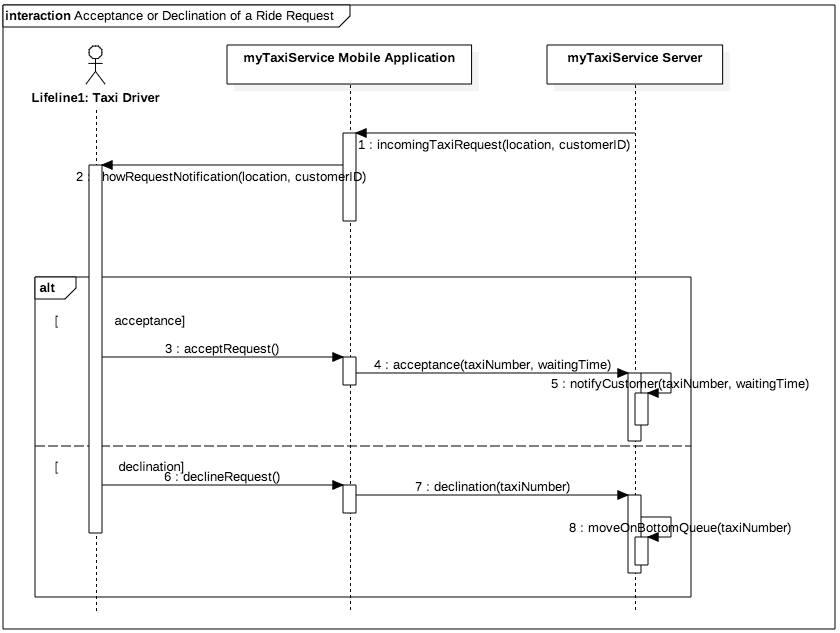
\includegraphics[width=\textwidth, scale=0.5]{IMG/InteractionDiagrams/AcceptDeclineRequest.png}
					\caption{Reservation Deletion Interaction Diagram}\label{sec:FigureAcceptDeclineRequest}
				\end{figure}